\documentclass{article}
\usepackage[english]{babel}
\usepackage{framed,graphicx,xcolor,hyperref}
\usepackage{tikz}
\setlength{\parskip}{10pt plus 1pt minus 1pt}
\author{Sander Koning, Florian Fikkert, Jacco Brandt, Joey Haas}
\date{\today}
\title{Integration project}
\usetikzlibrary{arrows}
\begin{document}
	\definecolor{shadecolor}{HTML}{A9A9F6}
	\maketitle
	\tableofcontents
	\newpage
	\section{Lorem Ipsum}
	\newpage
	\section{Dolor Sit Amet}
		\subsection{Initialization}
			The definition of the Distance-Vector routing protocol is as follows
			\footnote{\url{http://www.cs.bu.edu/fac/byers/courses/791/F99/scribe_notes/cs791-notes-990923.html}}:
			\begin{shaded}
				Lorem ipsum dolor sit amet, consectetur adipiscing elit. Vestibulum congue semper iaculis. Donec sagittis arcu eget elit congue, sit 					amet dapibus diam fermentum. Aenean lobortis eleifend nibh, et ornare mi varius eu. Praesent eu tellus lacinia, mollis nibh vitae, 					fringilla ligula. Donec ornare commodo fermentum. Cum sociis natoque penatibus et magnis dis parturient montes, nascetur ridiculus mus. 				Suspendisse nec elit risus. Duis quis facilisis urna, nec mattis quam. Phasellus faucibus, turpis et sagittis egestas, risus nibh congue 					tortor, rutrum varius orci mi vel ante. In sed imperdiet mauris. Fusce faucibus velit nec tortor tincidunt varius. Vivamus a nibh non 					enim pellentesque tempus porta ut turpis. Etiam facilisis eu lorem sed euismod.
			\end{shaded}

			Lorem ipsum dolor sit amet, consectetur adipiscing elit. Vestibulum congue semper iaculis. Donec sagittis arcu eget elit congue, sit amet dapibus diam fermentum. Aenean lobortis eleifend nibh, et ornare mi varius eu. Praesent eu tellus lacinia, mollis nibh vitae, fringilla ligula. Donec ornare commodo fermentum. Cum sociis natoque penatibus et magnis dis parturient montes, nascetur ridiculus mus. Suspendisse nec elit risus. Duis quis facilisis urna, nec mattis quam. Phasellus faucibus, turpis et sagittis egestas, risus nibh congue tortor, rutrum varius orci mi vel ante. In sed imperdiet mauris. Fusce faucibus velit nec tortor tincidunt varius. Vivamus a nibh non enim pellentesque tempus porta ut turpis. Etiam facilisis eu lorem sed euismod.

			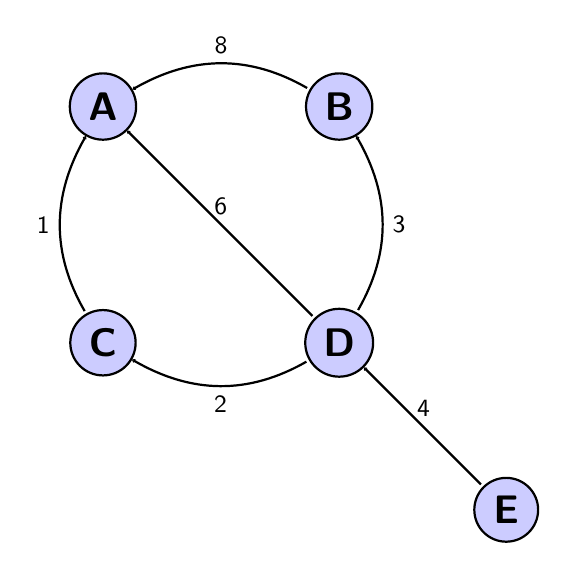
\begin{tikzpicture}[->,>=stealth',shorten >=1pt,auto,node distance=3cm,
				thick,main node/.style={circle,fill=blue!20,draw,font=\sffamily\Large\bfseries}]

				\node[main node] (1) {A};
				\node[main node] (2) [right of=1] {B};
				\node[main node] (3) [below of=1] {C};
				\node[main node] (4) [right of=3] {D};
				\node[main node] (5) [below right of=4] {E};

				\path[every node/.style={font=\sffamily\small},every arrow/.style=implies,implies-]
				(1) edge [bend left] node [above] {8} (2)
					edge [bend right] node [left] {1} (3)
					edge node [above] {6} (4)
				(2) edge [bend left] node [right] {3} (4)
				(3) edge [bend right] node [below] {2} (4)
				(4) edge node [above] {4} (5);

			\end{tikzpicture}
\end{document}
